\chapter{Desenvolvimento}

\section{Temas complementares}

\subsection{Promoção da produtividade}
\label{section: produtividade}

A produtividade (descrita como o quociente entre o trabalho realizado e os recursos utilizados), pode ser vista como a tradução da  eficiência de uma organização.


Esta é essencial para equipas de trabalho visto que sendo elevada, permite um rendimento superior numa menor janela temporal, impactando positivamente o cumprimento do planeamento efetuado.
  
Na Replai, a avaliação do desempenho dos seus colaboradores é obtida através de \textit{performance reviews} semestrais. 
Esta, realizada a nível de interpares e chefia.  
  
Quanto a interpares, tal como o nome indica, é pedido aos diferentes membros de uma equipa que façam uma heteroavaliação dos seus colegas de trabalho e expressem a sua opinião em relação ao valor do membro para a organização.  
  
Por exemplo, são colocadas questões sobre o fluxo do trabalho realizado, sobre o cumprimento dos objetivos delineados. Será a pessoa em questão um \textit{asset} para a equipa?
  
A informação é recolhida pela chefia e analisada. Consoante o rendimento, serão atribuídas compensações aos colaboradores da empresa.
  
Estas compensações podem exprimir-se sobre a forma de aumentos salariais diretos, bónus (\textit{one-time payout}).



\subsection{Economia Circular}
Desde a 1º revolução industrial, o modelo de produção e consumo adotado pelas empresas tem sido a Economia Linear. Baseia-se na premissa "Extrair, produzir, descartar".
\cite{EconomiaLinear}.

\begin{figure}[ht]
    \centering
    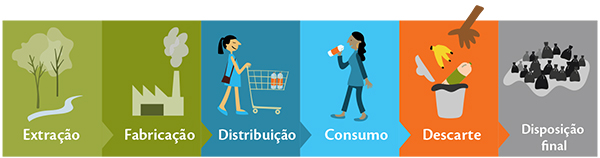
\includegraphics[width=10cm]{images/EconomiaLinear.png}
    \caption{Ilustração da Economia Linear}
    \UrlFont{bulbeenergia.com.br}
    \label{fig:economia_linear}
\end{figure}

Tendo em conta que as matérias-primas são finitas e o crescimento populacional é cada vez mais acelerado, torna-se evidente a necessidade de um novo modelo de produção, que vise o desenvolvimento sustentável invés da produção em massa.

Dessa necessidade, surgiu o conceito da Economia Circular. Tem por base os seguintes pressupostos: "redução, reutilização, recuperação e reciclagem de materiais e energia"\cite{EconomiaCircular}.

\begin{figure}[ht]
    \centering
    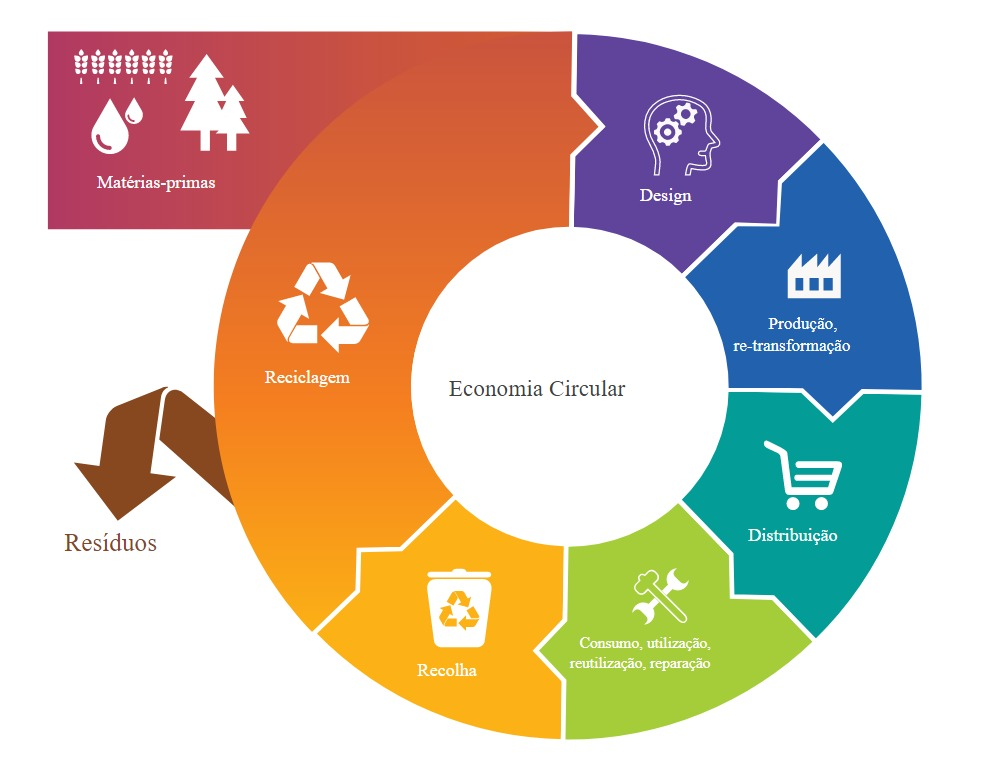
\includegraphics[width=7cm]{images/Economia_Circular.jpeg}
    \caption{Ilustração da Economia Circular}
    \UrlFont{www.europarl.europa.eu}
    \label{fig:economia_circular}
\end{figure}

Como podemos observar na Figura \ref{fig:economia_circular}, a economia circular espelha-se no ciclo dos ecossistemas. Para tal, os componentes técnicos dos produtos são planeados atempadamente com o intuito de serem facilmente reutilizados, renovados e atualizados\cite{EconomiaCircular1}. Graças a este maior planeamento, os produtos passam a ter uma vida útil maior. Por sua vez, faz decrescer a necessidade de uma produção em massa, reduzindo o lixo residual.

\begin{wrapfigure}[15]{l}{7cm}
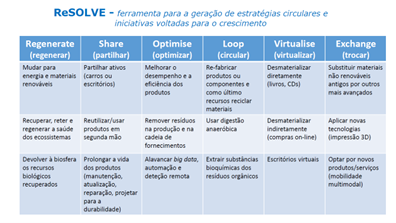
\includegraphics[width=7cm]{images/Resolve.png}
\caption{Tabela representativa das medidas que se enquadram nos pontos essenciais da Framework ReSOLVE.}\label{wrap-fig:1}
\UrlFont{moodle.isep.ipp.pt}
\end{wrapfigure}

Outro pilar fundamental da economia circular é o uso de energias renováveis e o respeito pela biodiversidade. Uma das ferramentas utilizadas para a geração de estratégias circulares e iniciativas voltadas para o crescimento é a \textit{framework ReSOLVE} \cite{EconomiaCircular1}. 

Com o intuito de conhecer melhor a Replai, perguntamos-lhe em quais pontos a empresa enquadra-se nos alicerces da filosofia ReSOLVE, obtivemos a seguinte resposta:\begin{quote}
"A Replai encaixa-se em dois pontos o \textit{Optimise} e o \textit{Virtualize}."\end{quote}

O conceito Optimise, visa a eficiência do produto desenvolvido. O produto desenvolvido pela Replai trata-se de um analisador de vídeos fazendo uso da inteligência artificial. Posto isso, o trabalho de análise anteriormente desenvolvido pelos colaboradores passa a ser da responsabilidade do software desenvolvido com a ajuda da inteligência artificial. Dessa forma, passamos a ter um processo automático e otimizado. 

Outro conceito em que a Replai se encaixa é o Virtualize. Visto que a empresa cria vídeos publicitários de acordo com as tendências do mercado, o processo criativo que antes era da responsabilidade dos colaboradores passa a ser da responsabilidade de um software com suportes tecnológicos. 

Tendo em conta que a empresa em questão desenvolve \textit{Software}, uma boa prática e sugestão seria focar no conceito de \textit{Share}. Esse conceito tem por base um maior ciclo de vida dos produtos desenvolvidos. Para que isso aconteça, a empresa necessita de um planeamento prévio do produto a ser desenvolvido para futuramente ser possível aplicar atualizações ao mesmo, conseguindo, dessa forma, prolongar o seu ciclo de vida e reduzir os gastos envolvidos na produção de um novo.

\section{Planeamento}
\subsection{Níveis de Gestão}
    Grande parte das empresas seguem a hierarquia de gestão apresentada na figura \ref{fig:hierarquia_gestao} e a Replai é uma delas. No entanto reparamos que diverge da regra geral.

    \begin{figure}[h]
        \centering
        \includegraphics[width=7cm]{images/Hierarquia de gestão.png}
        \caption{Níveis na Hierarquia de Gestão}
        \label{fig:hierarquia_gestao}
    \end{figure}

    Esta tem três gestores de topo, dos quais dois são fundadores da empresa. Um está responsável pelas vendas, \textit{Chief Sales Officer} (CSO), e o segundo fundador está responsável pelo produto, \textit{Chief Product Officer} (CPO). Por fim, o último gestor de topo é um \textit{Chief Director of Technology}.

    A empresa acredita que o conceito de gestores intermédios não traz benefícios à organização e dão o exemplo do jogo do telefone estragado, onde a mensagem da primeira pessoa chega ao fim da linha distorcida. Os gestores intermédios seriam mais um nível onde a mensagem iria diluir ou ficar presa. A informação deve fluir livremente entre camadas, e quantas mais houverem, mais resistência irá haver para que essa informação passe entre elas. Devido à dimensão da Replai, não existem recursos humanos nem gestores de \textit{financing}, logo, este trabalho é passado aos gestores de topo, e caso necessário, é efetuada por terceiros.
    
    Há varias equipas nas secção de vendas da Replai e cada equipa tem um diretor que é considerado gestor de primeira linha. Nas vendas, temos os \textit{Business Developers}, onde o seu maior objetivo é trazer fluxo de clientes que estejam interessados em comprar à Replai. Temos \textit{Account Management} que têm como objetivo manter clientes e impedir que estes cancelem o contrato. Existe também \textit{Customer Success}, que são responsáveis por um \textit{onboarding} eficaz dos clientes, ou seja, integrá-los devidamente na empresa, trabalhando lado a lado com os \textit{account managers}.
    
    Saindo das vendas, temos a secção da tecnologia: o \textit{Director of Technology}, que tem como objetivo reduzir ao máximo o número de \textit{bugs} e garantir a boa funcionalidade da plataforma e o \textit{Tech Lead Manager}, que vigia a qualidade do \textit{software} desenvolvido pela equipa.
    Por fim, o \textit{CPO} tem como objetivo manter a visão alinhada do produto e entregar as funcionalidades com mais alto impacto e menos custo. Dentro do produto, temos uma maior variedade de equipas que contêm funcionários não gestores. Por exemplo, o não gestor do \textit{design}, tem como objetivo resolver problemas e fazer o mínimo \textit{design} possível. Diogo afirmou que, tal como o \textit{Software Development}, um bom design é uma coisa que se deve que fazer pouco \textit{design}, ou seja, resolver os problemas com o mínimo de impacto possível. Os engenheiros têm como objetivo desenvolver requisitos de maneira a que se mantenham o mais sustentável possível e devem implementá-los com qualidade. Existe uma equipa de pesquisa que tem um \textit{Research Lead}, cujo objetivo é trazer informação que seja centrada no utilizador, ou seja, descobrir o que o utilizador realmente quer e é considerado a única área da empresa que não é influenciada.
    
    
\newpage
\subsection{Políticas de Planeamento}
    Sendo a Replai uma empresa voltada para área das tecnologias informáticas, a empresa organiza-se por equipas, que por sua vez adotam metodologias e tecnologias divergentes para organizar o seu trabalho. Um ponto em comum entre todas as equipas é a existência de um responsável por cada área de atuação da empresa. 
    
    \begin{wrapfigure}[16]{r}{6cm}
        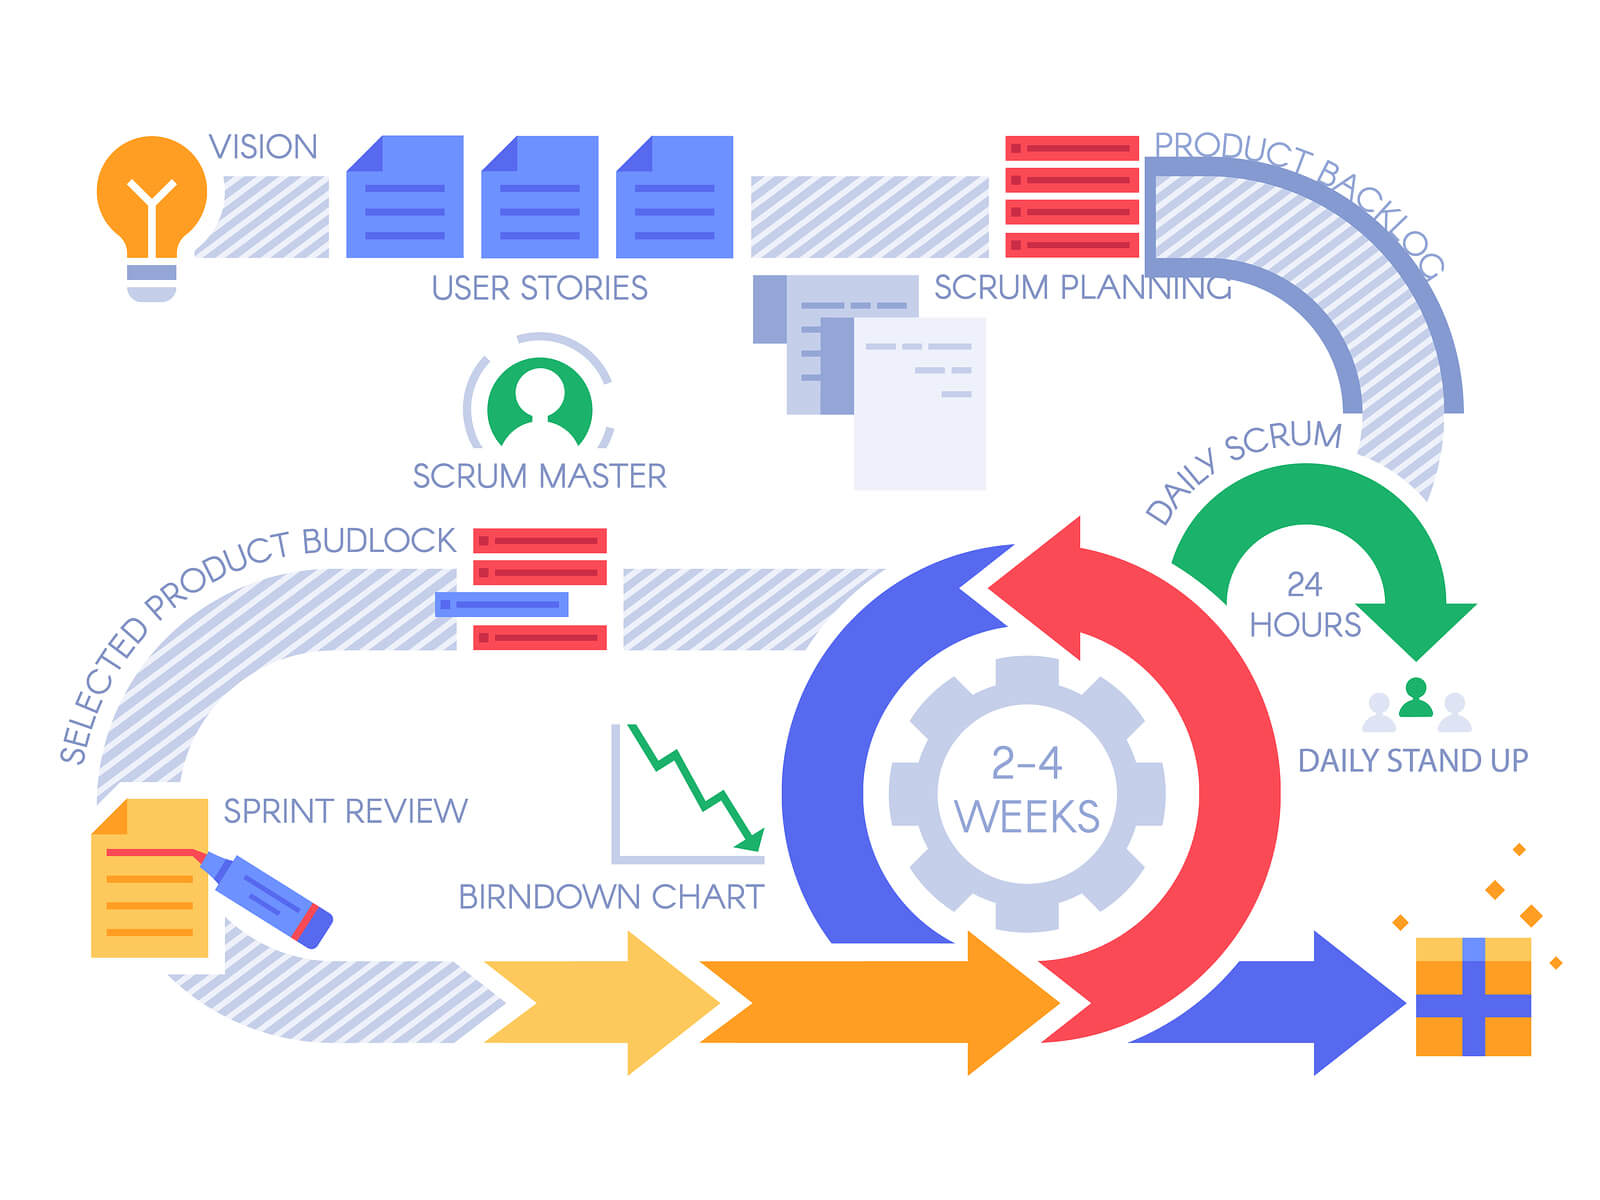
\includegraphics[width=5.5cm]{images/Innovación-ágil.png}
        \caption{Representação da metodologia Scrum.}\label{wrap-fig:2}
        \UrlFont{digite.com}
    \end{wrapfigure}
    
    A metodologia ágil adotada pela empresa é a Scrum. Caracteriza-se essencialmente pela divisão do trabalho em \textit{sprints}, realização de breves reuniões diárias e revisão do trabalho desenvolvido no término de cada \textit{sprint}. 
    
    Na Replai, os \textit{sprints} tem a duração de duas semanas. A distribuição de tarefas é feita usando os casos de uso do sistema, porém, os funcionários também podem exercer tarefas de investigação. Caso os colaboradores possuam tarefas de investigação recebem uma menor quantidade de casos de uso, para que não haja sobrecarga.
    
    Depois de feita a distribuição das tarefas, cada equipa faz uso de ferramentas específicas para gerenciar o seu trabalho. Por exemplo, a equipe de venda faz uso do \textit{software} HubSpot para organizar o plano de vendas da empresa e manter o registo dos potenciais clientes. Já a equipe de desenvolvimento faz uso da ferramenta Jira, que permite gerir a distribuição dos casos de uso entre os colaboradores e no final de cada \textit{sprint} gerar gráficos que são pertinentes para analisar e debater o trabalho desenvolvido até o momento e refletir sobre as boas ou más práticas que devem ser mantidas ou alteradas para o próximo \textit{sprint}.  
    
    No final do desenvolvimento de cada projeto é feito um gráfico da velocidade de produção. Esse gráfico é a razão entre o número de casos de uso finalizados em todos os \textit{sprints} sob a número de \textit{sprints}. A partir desse resultado é possível planear/ajustar os projetos com base na média de trabalho das equipas.

\subsection{Planeamento Organizacional}

As equipas de trabalho, para desenvolvimento de software, recorrem à metodologia Agile Scrum. As user stories são definidas como objetivos claros e mensuráveis, de forma a permitir alcançar as metas definidas, story points.
  
Contudo, para tarefas que podem requerer, por exemplo, investigação, recorrem a time boxes, que permitem alocar uma quantidade fixa e máxima de recursos que poderão ser dedicados a uma dada tarefa.
  
Como dito pelo Diogo na entrevista, se uma determinada tarefa não for de fácil análise e não for possível mensurar a mesma, esta irá prejudicar o fluxo da equipa e, também, demonstrará que a divisão do trabalho necessário não foi efetuada corretamente.


\subsection{Valores, Visão e Missão da Replai}

Como mencionado na caracterização, o serviço prestado pela Replai é diferente da visão inicial, visto que o mesmo possuía certas falhas.

Apesar de a visão da empresa ter sido ligeiramente alterada, a sua missão e o seu plano estratégico (transição governamental para empresarial) baseia-se na mesma ideia: perceber como um vídeo funciona! Desta forma a visão da Replai é ser um fator essencial nas empresas do mundo \textit{gaming} criarem a cultura mais enriquecida no mundo dos \textit{esports}. A missão da Replai é ajudar as empresas a aumentar a adesão, lealdade, e entusiasmo dos amantes de \textit{gaming} perante a sua marca \textit{esports}.

A empresa descreve-se como sendo desafiante, destemida, dedicados ao desenvolvimento do melhor produto e extremamente abertos a ideias novas, sugestões e uma comunidade saudável para poderem ter um excelente ambiente de trabalho!

\subsection{Cadeia de Valor}
A cadeia de valor caracteriza-se como sendo o processo de agregar valor as atividades desenvolvidas pela empresa, seja ela a confeção de novos produtos ou serviços. 

\ Esse processo tem como principal função ajudar as empresas a compreenderem o seu funcionamento e por consequência, melhorar o seu processo produtivo.
Para compreendermos melhor como a cadeia de valor funciona, Michael Porter criou uma divisão teórica que nos ajuda a compreender esse processo. Para tal, subdividiu o processo em dois tipos de atividades: primárias e de suporte\cite{CadeiaDeValor1}.

\ As atividades primárias também chamadas de processos \textit{Core}, são todas aquelas que geram benefícios diretos para os clientes. Essas atividades são as seguintes:\\

\textbf{-Logística de entrada:}  Refere-se ao relacionamento com fornecedores, aquisição de matéria-prima e contratações de serviços.\\

\textbf{-Operações:} Refere-se ao processo de criação de um produto ou serviço.\\

\textbf{-Logística de saída:} Refere-se as atividades de entrega do produto/serviço ao consumidor final.\\

\textbf{-Marketing e vendas:} Refere-se aos processos utilizados para atrair consumidores. \\

\textbf{-Serviços:} Refere-se as atividades de suporte ao produto/serviço.\\

\ Tendo por base esses conceitos, iremos analisar as atividades primárias realizadas pela Replai. 

\ Em relação a Logística de entrada, sendo a empresa voltada para a área de informática, a “matéria-prima” utilizada para a criação dos seus produtos são novas ideias e pesquisas. 

\ Referente as Operações, a Replai divide a criação de um produto/serviço em 4 etapas: Análise, Pré-Planeamento, Refinamento e Planeamento e Execução. Cada uma dessas fases é caracterizada por inputs e outputs expectáveis, como representado na figura abaixo.
    \begin{figure}[ht]
       \centering
        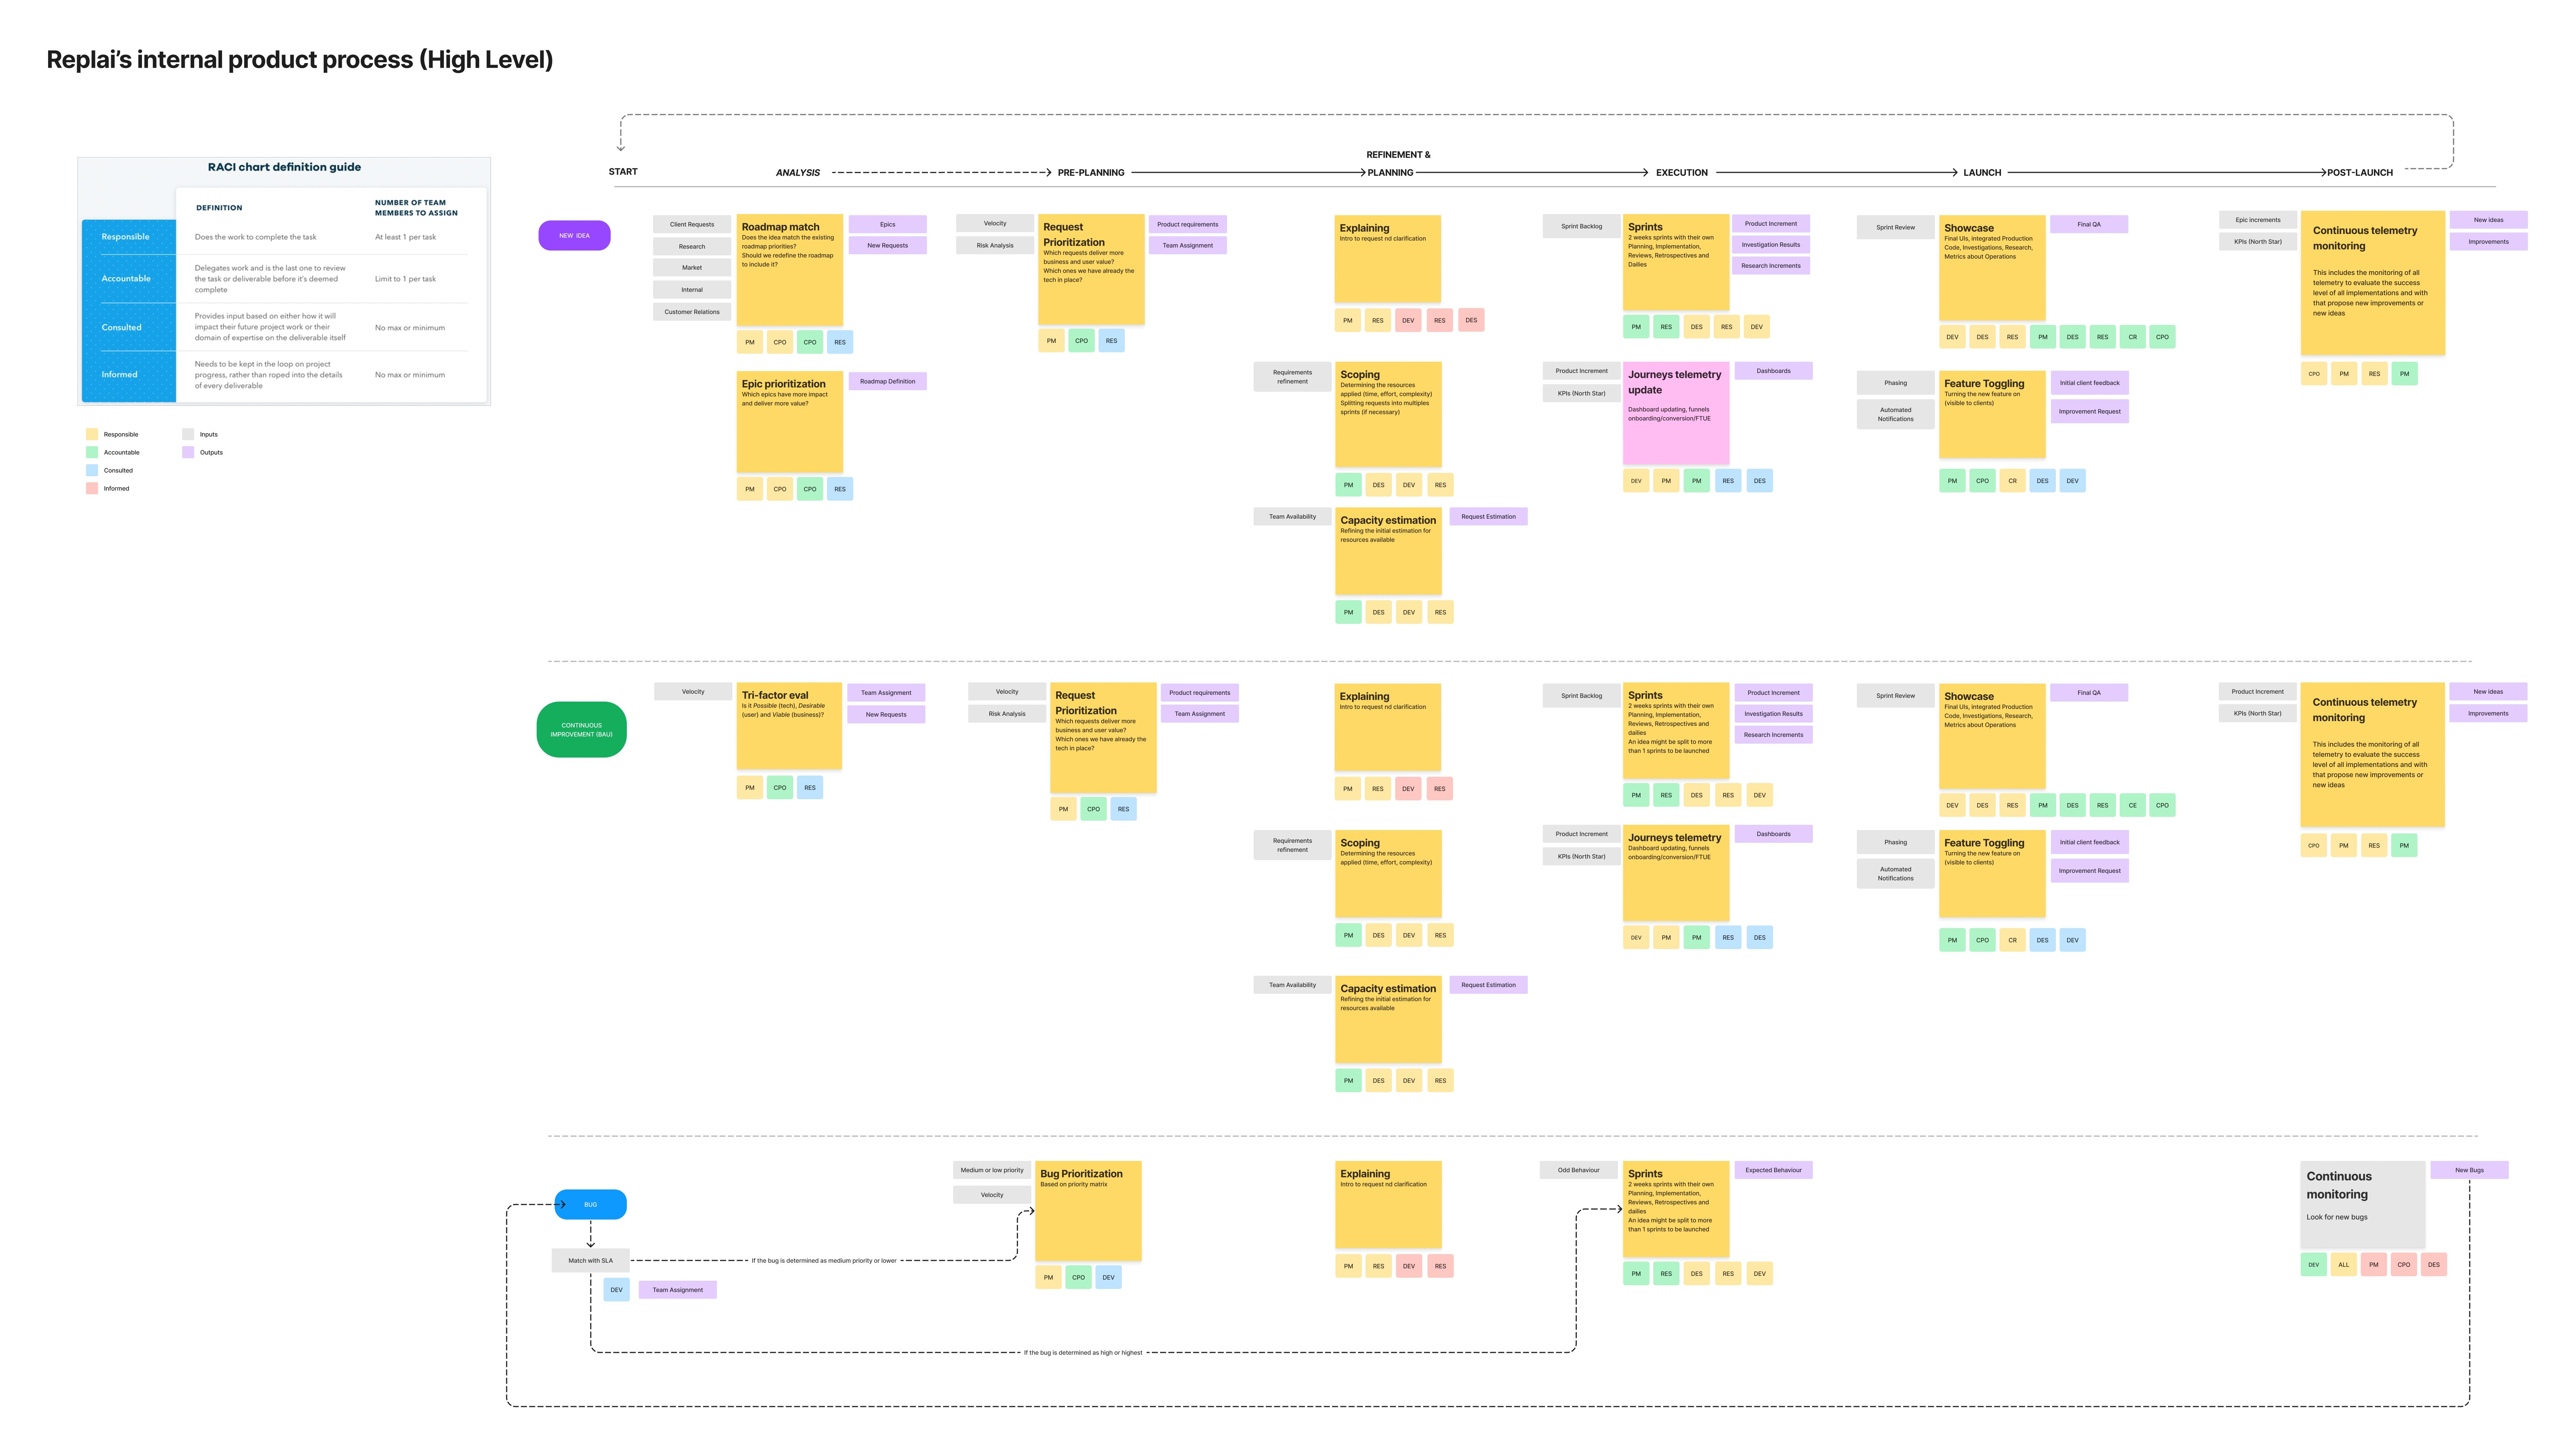
\includegraphics[width=11cm]{images/Replai-Process.jpg}
        \caption{Etapas de desenvolvimento de um projeto na Replai.}
        \label{fig:replai_processo}
    \end{figure}\\

\ Passando ao ponto referente a Logística de saída esse é feita de forma totalmente virtual visto que e empresa desenvolve Software.

\ Relativamente as estratégias de Marketing utilizadas pela empresa, as principais são: a divulgação de novos produtos pelas redes sociais e a estratégia de libertar novas funcionalidades em fases e com públicos alvos específicos, para conseguir captar a atenção e despertar interesse continuo pelo produto.

\ Por último temos os Serviços, na Replai existe uma equipa de suporte para atender a eventuais problemas relacionados com o produto adquirido pelos seus clientes.\\

\ Já as atividades de suporte caracterizam-se por gerarem valor indiretamente para empresa pois, dão suporte as atividades primárias\cite{CadeiaDeValor}.Essas atividades são as seguintes:\\

\textbf{-Infraestrutura:} Refere-se a gestão administrativa, legal e financeira\cite{CadeiaDeValor} da empresa.\\

\textbf{-Gestão de Recursos Humanos:} Refere-se ao processo de aquisição de novos colaboradores e capacitação dos já existentes.\\

\textbf{-Desenvolvimento Tecnológico:} Refere-se a automatização dos processos da empresa. \\

\textbf{-Aquisição/compras:} Refere-se essencialmente a negociação com os fornecedores e busca de matérias-primas.\\

\ Tendo por base esses conceitos, iremos analisar as atividades de apoio realizadas pela Replai.

\ Em relação a Infraestrutura, a gestão legal e financeira é feita através de serviços terceirizados.

\ Quanto aos recursos humanos, atualmente está a cargo do fundador da Replai, sendo este o responsável pela contratação de novos colaboradores assim como oferecer formação continua aos seus empregados atuais.

\ Relativamente a automatização de processos, a Replai possui uma política de contratação de \textit{freelancers} para desenvolverem tarefas genéricas que não envolvam o contexto de domínio de negócio do projeto que está a ser desenvolvido. Dessa forma, otimizam o seu trabalho, podendo aplicar o seu tempo em tarefas mais complexas.

\ Passando ao último ponto, A aquisição/compra, sendo a Replai uma empresa voltada ao desenvolvimento de \textit{software}, não existe grande relação com fornecedores e compra de matéria-prima. 





\subsection{Análise do ambiente competitivo}
\begin{quote}
    "Uma organização é sempre inseparável do espaço em que se coloca"\cite{Planeamento}
\end{quote} e portanto, é importante fazer uma análise dos fatores externos e internos nos quais podem por em causa o sucesso da empresa. A investigação e análise constante destas características  é o que possibilita as empresas permanecerem competitivas na sua longevidade. A este conjunto de fatores no ambiente externo com os fatores do ambiente interno denomina-se ambiente competitivo.

Para uma melhor compreensão dos ambientes que coexistem no espaço da empresa, identificasse três tipos de ambientes: \\

	\textbf{-Ambiente externo geral:} Neste ambiente são analisados fatores que estão fora do controlo direto da empresa. Estes elementos são características que todas as organizações do mundo enfrentam, independentemente do seu setor de atividade. \\
	

	\textbf{-Ambiente externo especifico:} O ambiente externo específico avalia o grau de competitividade do setor que uma organização está ou se pretende colocar.  Neste ambiente qualifica-se o grau de atratividade assim como se analisa indicadores de entrada ou saída do mercado.\\

	\textbf{-Ambiente interno:} Em suma, o ambiente interno é o responsável pela análise do sucesso e funcionamento da organização, isto é, que vantagens competitivas e fraquezas a organização apresenta para o mercado do setor de atividade em que se encontram. \\
	
	
\newpage
\subsubsection{Análise PEST}
Para análise do ambiente externo geral recorre-se a uma ferramenta denominada Análise PEST. Sendo PEST um acrónimo resultante do acoplamento das iniciais: Políticos (P), Económicos (E), Sociais(S), Tecnológicos (T). \\

%Dito isto,"PEST" refere-se respetivamente a: \\


\noindent \textbf{Fatores políticos} %, fatores que incluem questões legais e regulamentares como por exemplo, Política Fiscal e Regulações Ambientais.
\begin{itemize}
    \item A Replai, sendo uma empresa sem sede, no entanto, multinacional, está dependentes das políticas fiscais relacionadas com empresas digitais e e-commerce.
    \item Como a empresa tem clientes por todo mundo, é necessária uma elevada atenção à legislação e estabilidade governamental dos países colaboradores.
\end{itemize}

\underline{Exemplos Práticos}:
\begin{itemize}
    \item Devido à guerra, e sendo que a Replai tem colaboradores ucranianos, alguns clientes viram-se forçados a desistir e deixar de usufruir dos produtos da empresa.
    \item Consequentemente os conflitos políticos dificulta a adesão de clientes russos e/ou ucranianos \\
\end{itemize}


\noindent \textbf{Fatores Económicos} %, estes abordam o poder de compra da organização e o custo capital, para analisar temos que verificar que efeitos, por exemplo, de que forma as taxas de câmbio, inflação  juros afetam a empresa.
\begin{itemize}
    \item Como a Replai se sustenta através de rondas de investimentos, esta está  sujeita ás condições presentes na legislação relativa a investimentos.
    \item Altamente suscetíveis à inflação e ao valor que os investidores atribuem à Replai.
\end{itemize}

\underline{Exemplos Práticos}:
\begin{itemize}
    \item A Replai sustenta-se através de rondas de investimento. Devido à recessão atual derivado da pandemia e da guerra, uma das rondas de investimento não foi concretizada apesar dos resultados obtidos pela empresa, isto resultou numa mudança de estratégia de sustento da empresa de \textit{hypergrowth}, para cobrir despesas primeiro e assegurar lucros.\\
\end{itemize}


\noindent \textbf{Fatores Sociais} %, que incluem fatores culturais e distribuições geográficas da organização, inclui exemplos como estilos de vida, hábitos consumo e distribuição etária. \\
\begin{itemize}
    \item A faixa etária consumidora de vídeos tem alargado, um ponto fulcral para a Replai pois origina mais possíveis clientes.
    \item Está presente na era digital, onde o consumo de vídeos é abundante.\\
\end{itemize}

\noindent \textbf{Fatores Tecnológicos} %, o fator que aborda a terceirização da empresa. Avaliada através dos processos de investigação e automação da empresa. \\
\begin{itemize}
    \item A possibilidade de inovação tecnológica neste ramo é alta, pois é um mercado pouco saturado.
    \item A possibilidade de evolução tecnológica em produtos já existentes é igualmente elevada, já que há muita procura e pouca oferta. 
\end{itemize}

\underline{Exemplos Práticos}:
\begin{itemize}
    \item Tiktok, a plataforma de partilha e criação de vídeos curtos, lançou recentemente um algoritmo avançado de estudo de tendências e métricas relevantes para o sucesso de publicidades. Isto inicialmente apresentou-se como uma ameaça, no entanto, como a Replai se especializa no mercado gaming, acabou por não ser afetada totalmente.
\end{itemize}
\newpage
\subsubsection{Análise de Porter}
Questionamos o Diogo, \textit{Project Manager}, relativamente ao modelo das cinco forças de Porter, como mostra a figura \ref{fig:Porter}, e como ele avalia essas forças no impacto da rendibilidade da organização.

\begin{figure}[ht]
    \centering
        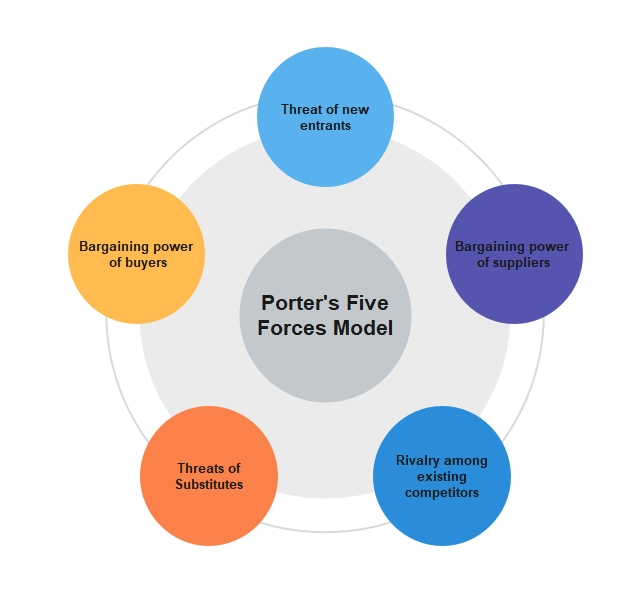
\includegraphics[width=10cm]{images/porters-five-forces-model.jpg}
        \caption{Cinco forças de Porter}
        \label{fig:Porter}
\end{figure}

\noindent\textbf{Rivalidade entre os concorrentes existentes:}\\

O espaço onde a Replai se encontra ainda está muito inexplorado, logo todas as empresas, que são poucas, estão à caça do \textit{market share}. Todas as abordagens entre os concorrentes são muito parecidas. Apesar do Diogo ser influenciado, afirma que a Replai tem uma abordagem muito diferenciadora da concorrência, à parte de uma outra empresa. Esta é a que tem mais sucesso nesta competição, está muito avançada, mas é vista pelo Diogo como sendo uma parte adjacente a todo o processo e não um concorrente direto. 

Concluímos com o Diogo que o facto de serem poucas empresas é uma força \underline{Fraca}, e também tivemos em conta que todas as empresas estão à procura do maior market share possível, o que consideramos ser uma \underline{Grande} força. Logo a força que o Diogo usou para caracterizar a rivalidade entre os concorrentes existentes foi \textbf{\underline{Moderada}}.\\

\noindent\textbf{Poder negocial dos fornecedores:}\\

A Replai sendo uma empresa de software, de momento tem o único fornecedor, a Amazon. Como esta empresa, há muitas que oferecem os mesmos serviços. Mudar de fornecedor também é extremamente fácil e sem qualquer custo para a empresa a não ser o custo de serviço.

Sendo assim, chegamos a uma rápida conclusão com o Diogo. Haverem muitas empresas a fornecerem o mesmo serviço é, para a Replai, uma força \underline{Fraca}, e a facilidade de como podem alterar de fornecedor é também uma força \underline{Fraca}, sendo então o Poder negocial dos fornecedores, uma força \textbf{\underline{Fraca}}.\\

\newpage
\noindent\textbf{Ameaça de novos concorrentes:}\\

Foi-nos falado de um momento importante na história que marcou o mercado da Replai. A Apple removeu um identificador dos iPhones com o iOS14, identificador que dava o perfil do utilizador, no que conta a publicidade. Sendo este removido, muitas empresas que queriam conhecer os seus clientes para lhes fornecer publicidades ficaram sem forma de o fazer, criando assim, uma grande procura em empresas como a Replai. Cada vez mais surgem novas empresas a tentar fazer exatamente o mesmo que ela faz. O Diogo contou-nos que já há algum feedback do que corre mal e do que corre bem, mas que não há solução perfeita. Solução esta que de acordo com ele não existe, deu como exemplo a Google, que não é uma solução perfeita, mas é uma solução ótima. 

Neste mercado da Replai ainda não existe uma solução ótima, e há sempre uma chance moderada de um novo concorrente encontrar essa solução, Diogo classifica este facto como sendo uma força \underline{Forte}. Como este mercado está a ter cada vez mais procura, o Diogo vê o aparecimento de muitas novas empresas como uma força \underline{Forte}. Concluindo assim que a ameaça de novos concorrentes é uma força \textbf{\underline{Forte}}.\\

\noindent\textbf{Poder negocial dos clientes:}\\

O mercado da Replai é maioritariamente \textit{Business to Business}, logo os clientes são entidades, o que significa que há um numero baixo de clientes, sendo eles todos muitos importantes para a empresa. O Diogo deu-nos exemplos de grandes empresas que são seus clientes como a Activision, a Zinga, Rovio, entre muitos outros, e perder esse clientes vinha com um grande custo para a Replai.

Tendo isto tudo em conta, depreendemos que ao haver muitos poucos clientes, estes tem uma \underline{Grande} força no poder negocial. Da forma que o mercado da Replai funciona, todos os clientes são grandes empresas, o que faz delas clientes muito importantes, fazendo com que estes tenham também uma \underline{Forte} força. Em suma o poder negocial dos clientes é caracterizado como sendo, uma força \textbf{\underline{Forte}}.\\

\noindent\textbf{Ameaça de produtos substitutos:}\\

O Diogo diz que a Replai é das empresas mais caras, senão a mais cara. Apesar dos seus cliente serem maioritariamente grandes organizações, ou indivíduos com grande poder de compra, existe sempre a preocupação dos clientes tenderem para produtos mais baratos. Para contrariar esta preocupação, sabe-se que nenhum outro produto é considerado a solução ótima, como já foi previamente referido, então não há garantias de que os esses produtos possa substituir o que a Replai tenha para oferecer. O Diogo confirma também que esta é muito diferenciadora em comparação com a competição.

Concluímos assim que há uma \underline{Grande} força que afeta a Replai por eles serem dos produtos mais caros no mercado, por outro lado, não se pode dizer que as outras empresas a possam substituir, logo o Diogo considera que este aspeto tenha uma \underline{Fraca} força. Fazendo, por fim, com que a ameaça de produtos substitutos seja uma força \textbf{\underline{Moderada}} para a Replai.\\

\newpage
\subsubsection{Análise VRIO}

O modelo VRIO (Valor, Raridade, Imitabilidade e Organização, respetivamente) permite avaliar \textit{assets} de uma determinada empresa, ao sujeitarmos a qualidade em questão a estes 4 parâmetros.
  
Iremos usar o seu algoritmo e a capacidade de organização e adaptabilidade como recurso e competência, respetivamente, no estudo através desta \textit{framework}.\\

\begin{figure}[ht]
    \centering
        
\includegraphics[width=7cm]{images/vrio.png}
        \caption{Framework VRIO}
        \label{fig:vrio}
\end{figure}

\noindent \textbf{Recurso:} \\

\noindent \textbf{Valor}\\
 
O algoritmo por trás do produto da Replai é, possivelmente o seu recurso mais forte. Através do  mesmo, a empresa consegue vender as métricas e os marcadores que representam a análise dos conteúdos dos consumidores.
  
Numa sociedade em que quotidianamente, a expansão do consumo de vídeo dá-se exponencialmente, seja para empresas ou criadores de conteúdo, o sucesso do vídeo, por exemplo, a nível publicitário, é um fator para a expansão de uma determinada organização.\\

\noindent \textbf{Raridade e Imitabilidade}\\

Dado que foi desenvolvido pioneiramente e permanece com um resultado único no mercado, o mesmo é também raro e imitável, visto que se encontra patenteado. Existem produtos com princípios de funcionamento semelhantes, contudo, com uma visão de análise distinta da Replai.\\

\noindent \textbf{Organização}\\
  
Aproveitando o seu recurso exclusivo, a empresa facilita o acesso ao mesmo por parte do utilizador. Faz isso através de interfaces simples, interpretação em temo real e uma integração profunda do seu produto com as maiores plataformas de vídeo, como o Youtube.
  
A remoção do atrito entre a disposição de resultados e a interpretação dos utilizadores por meio de diagramas e painéis de utilizador permitem uma experiência autónoma e intuitiva.\\

\noindent \textbf{Competência:}\\

\noindent \textbf{Valor}\\

Desde a sua fundação que tinha como visão serem uma empresa \textit{user centered} e com um workflow estruturado, algo essencial em ambiente de \textit{start-up}, dado que os recursos são limitados. Não só isso, mas equipas devidamente geridas e com objetivos claros e atingíveis, são propensas a uma produtividade e motivação superior, beneficiando o projeto em que trabalham.\\

\noindent \textbf{Raridade e Imitabilidade}\\
  
Como descrito pelo PMO, Diogo Bastos, engenheiros com experiência prévia em grandes centros tecnológicos, tais como \textit{Silicon Valley}, ficaram admirados com a capacidade da Replai.

Considera-se um recurso raro, dado que grandes empresas fazem uso do dinheiro de forma a resolver os problema sem solução para o causador.\\

\noindent \textbf{Organização}\\

Apesar de raro, é possivelmente imitável, contudo, apenas através de boa gestão. Assim, demonstra-se a capacidade organização desta pequena empresa, que impulsiona os “tubarões” da indústria tecnológica (e não só)! 
 

\subsubsection{Análise SWOT}
Com base no que aprendemos até agora, realizamos em conjunto uma análise SWOT da Replai na figura \ref{fig:swot}.\\
\begin{figure}[ht]
    \hspace*{-2.5cm}   
    \centering
    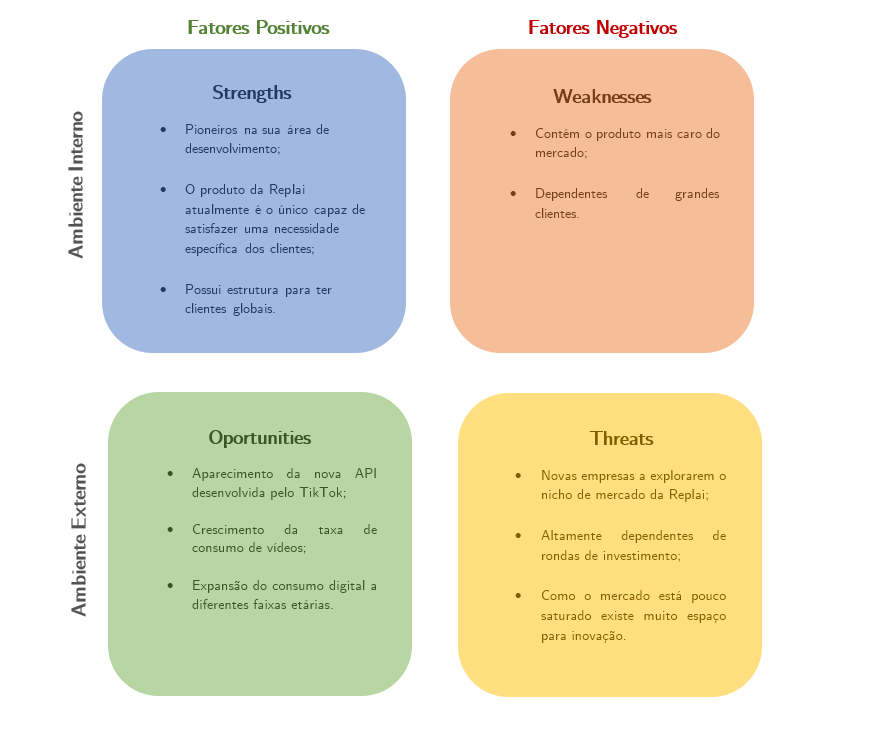
\includegraphics[scale=0.8]{images/SWOT.png}
    \caption{Análise SWOT}
    \label{fig:swot}
\end{figure}

\newpage
\subsection{Possível Estratégia da Organização}
Segundo o processo de planeamento estratégico apresentado na figura \ref{fig:planeamento}, o único ponto que sugerimos uma melhor abordagem é na formulação de objetivos. Apesar da Replai ter objetivos definidos, estes objetivos não estão de acordo com a ferramenta SMART, principalmente no \textit{\textbf{T}}, o ponto temporal. Todos os objetivos são específicos, mensuráveis, atingíveis, e relevantes, nenhum deles nos foi apresentado com uma data de alcance.

\begin{figure}[ht]
    \centering
    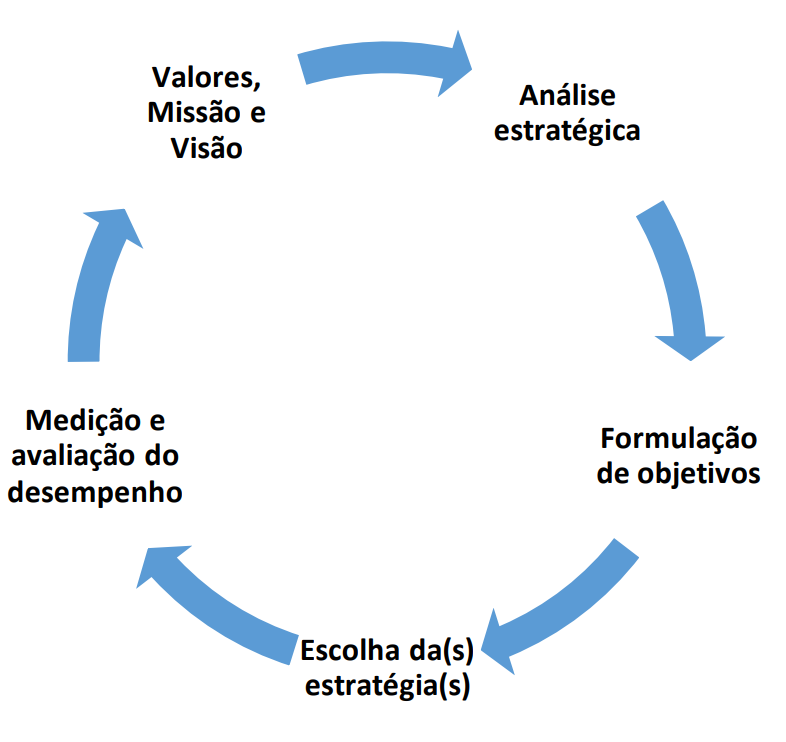
\includegraphics[scale=0.5]{images/planeamento.png}
    \caption{O processo de planeamento estratégico}
    \label{fig:planeamento}
\end{figure}


Perante a análise estratégica, e adaptando ligeiramente os valores, a missão, e a visão da Replai, propomos a seguinte estratégia. Expandir para um novo mercado, possivelmente cinema, já que este tem um publico maior e tem surgido uma interligação entre estes dois setores, para deixarem de estar dependentes de grandes clientes num mercado ainda restringido.

\newpage    
\section{Organização}
\subsection{Análise do organograma da organização: tipo de departamentalização, flexibilidade, número de níveis hierárquicos, posições de linha e de staff}

Após efetuar-se uma análise detalhada do organograma, é possível confirmar que o tipo de departamentalização da Replai é Organizacional funcional. Não só isso, como também foi possível tirar as conclusões que vão ser detalhadas posteriormente.
  
A departamentalização, sintetizada como o agrupamento de unidades lógicas e funcionais, é essencial para uma organização conseguir atingir os objetivos definidos na estratégia adotada. Antes de verificarmos a departamentalização desta empresa, é preciso verificar o número de níveis hierárquicos e a forma como são constituídos.
  
O esquema que nos foi fornecido está dividido em 2 árvores hierárquicas principais, que caracterizam a equipa de desenvolvimento e a equipa de marketing. Estas possuem 5 e 3 níveis hierárquicos, respetivamente, algo que é frequente nos modelos de gestão atuais, caracterizados pela fomentação no que toca à delegação de autoridade, originando estruturas deveras flexíveis e ágeis. É possível verificar que, ao contrário de habituais estruturas de gestão, devido ao facto de a gestão intermédia, quando precisa, ser \textit{outsourced}, o reduzido número de pessoal e a preferência por menos camadas, contribui para que o número de patamares seja reduzido.
  
Por exemplo, nos níveis imediatamente inferiores ao do CPO, é possível verificar a existência de cargos como \textit{UX Researcher} ou \textit{Product Manager}, que se aproximam mais do âmbito técnico. Porém, apesar de a estrutura da Replai ser horizontal e descentralizada, reúne um conjunto de desvantagens, como o elevado atrito na comunicação dentro do próprio nível (dado que este é “achatado”).
 
Devido ao facto de ser uma organização de dimensão reduzida (com menos de 50 trabalhadores), é possível verificar a existência de cargos que ocupam posições de linha, como indicado pelos níveis de gestão da empresa. Gestores de topo (\textit{CSO, CPO e Chief Director of Technology}), uma gestão intermédia \textit{outsourced} e, no nível inferior, funcionários não gestores (considerados \textit{staff}), totalizando 3 níveis de encargos agrupados. 
  
Como as atividades desempenhadas em cada nível são semelhantes (daí a formação de grupos), pode-se dizer que a estrutura é funcional. Porém, a resposta a esta caracterização não é tão linear como aparenta. Esse impasse deve-se ao facto de a sua estrutura intermédia ser \textit{outsourced} (desempenhado por terceiros) e esta componente ser indesejada pois, como mencionado previamente, é vista como uma forma de difusão da informação que se deseja transmitir entre camadas.
  
Não só isso, mas também se deve ao facto de certos módulos de uma departamentalização divisional poder ser efetuada. Como mencionado durante a entrevista, com o objetivo de poder fornecer uma experiência mais personalizada e adaptada ao cliente em questão, alguns funcionários já viajaram de forma a poder estar mais perto do cliente e, assim, poder adequar o serviço prestado às necessidades do mesmo. Devido a serem ocorrências limitadas e esporádicas, não é possível considerar que fazem parte da estrutura habitual da empresa.
  
Assim, elimina-se também a opção de uma estrutura mista.

\begin{figure}[ht]
    \centering
    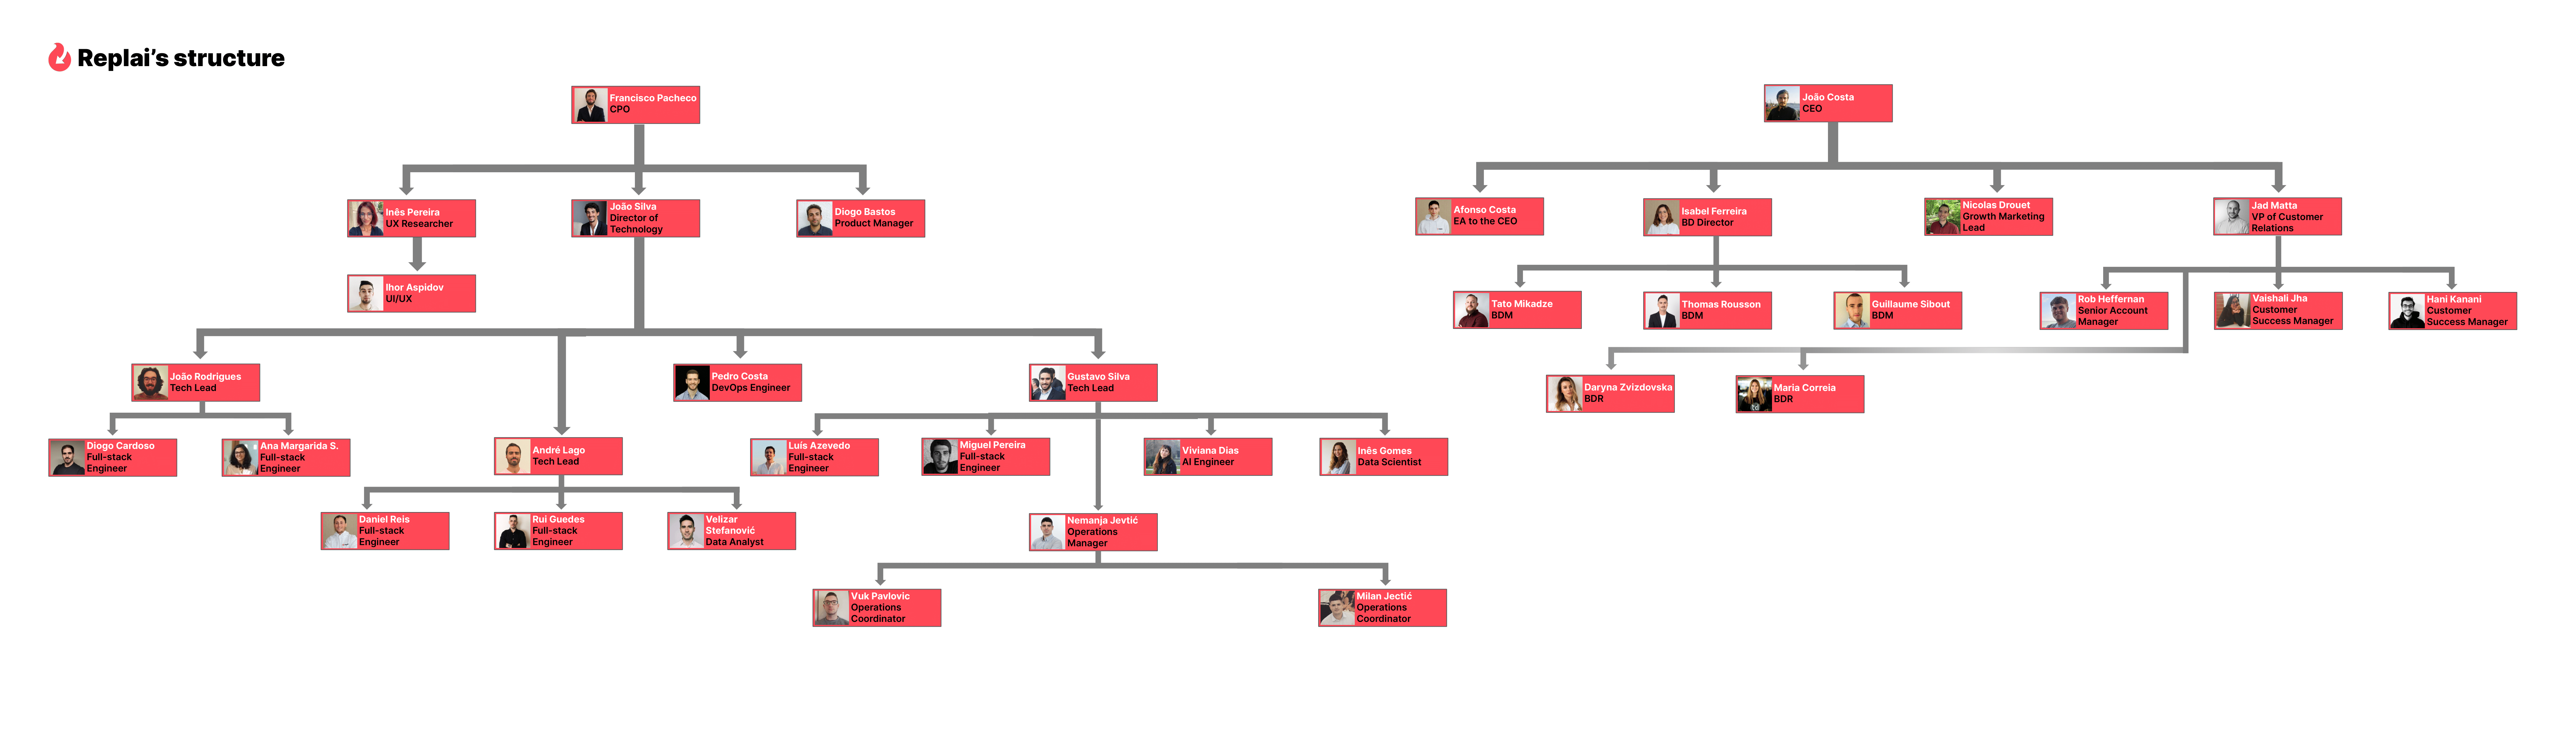
\includegraphics[width=15cm]{images/organograma.png}
    \caption{Organograma}
    \label{fig:organograma}
\end{figure}

\subsection{Análise da Organização Formal e Informal da Empresa}

Em relação a organização formal, identificamos que o departamento mais formal dentro a empresa é o de Marketing. Pois, esse é responsável pela comunicação direta com os consumidores. Existe também um cuidado em registar essa comunicação para que haja um controle de informação. \\

Já em relação a organização informal, pelo colaboradores possuírem uma grande autonomia decisional, principalmente a equipa de \textit{Tech}, não existe uma imposição hierárquica muito forte em relação as tarefas específicas a serem realizadas por cada departamento.
Outro ponto a mencionar é a realização de atividades de desporto entre os colaboradores. Eles possuem um grupo de padel, tênis e futebol e reúnem-se quinzenalmente para praticarem atividades e melhorarem a relação fora do ambiente de trabalho.No fim do ano, realizam também uma viagem em conjunto.


\subsection{Comentário breve à estrutura organizacional}
Segundo a análise do organograma podemos perceber que a Replai opta por uma estrutura mais achatada. Este tipo de estrutura permite delegar mais responsabilidades a cada colaborador, assim como facilita a adaptação e melhora a flexibilidade. 
Como grupo acreditamos que esta estrutura faz sentido no contexto da Replai, pois tendo em consideração a dimensão da empresa, o ideal será dar o máximo autonomia possível aos colaboradores. No entanto, devido a esta estrutura, torna-se mais evidente a necessidade de colaboradores com conhecimento em diversas áreas. 

\subsection{Reflexão sobre a possibilidade da alteração do tipo de departamentalização}

Atualmente, a Replai tem apenas um tipo do produto, os seus clientes encontram-se em diversos países e são grandes empresas. Contudo, a Replai tem poucos funcionários, devido a isto, consideramos que o atual tipo de departamentalização (Estrutura organizacional funcional) é o ideal para a empresa. Num possível futuro onde Replai tem uma maior dimensão, recomendaríamos adaptar a estrutura organizacional divisional por áreas geográficas pois estar geograficamente perto dos clientes pode facilitar a coordenação das atividades.


\newpage
\section{Controlo de gestão}

\subsection{Principais sistemas de controlo de gestão}

O controlo de gestão principal basiea-se num sistema de avaliação de desempenho e é muito simples, é feita uma \textit{performance review} do colaborador. Esta baseia-se em recolher \textit{feedback} das pessoas mais próximas, por exemplo, programadores terão \textit{feedback} dos outros programadores e da chefia direta. São feitas três perguntas neste \textit{feedback}, "O que se está a fazer bem?", "O que se tem de melhorar?", "Porque é que se é uma mais valia para a empresa?". Depois destas três perguntas, deve ser feita uma auto avaliação. 

Deve-se também esclarecer objetivos até a próxima \textit{performance review}, por exemplo, fazer uma viagem para estar com um cliente real. Existirá uma sessão com a chefia direta onde se apresentará esta \textit{performance review}, discutir-se-ão pontos e vai-se arranjar \textit{action items} (tarefas) para se resolver assuntos importantes.

Na próxima \textit{performance review} começa-se com a avaliação da anterior com a intenção de analisar se houve melhorias onde nos comprometemos. Estas \textit{performance reviews} acontecem de meio em meio ano, mas existem \textit{1 on 1s} com a chefia mais frequentemente, uma vez a cada duas semanas, ou até uma vez por semana. Estes \textit{1 on 1s} são para se ter feedback mais recorrente.

Outros sistemas de controlo de gestão que são utilizados nos diversos níveis de gestão da empresa incluem o sistema de orçamento de capital, que é um processo pelo qual a empresa planeia e controla o seu uso de recursos financeiros para atingir os seus objetivos.  Também é utilizam um sistema de gestão de produção para monitorizar e controlar a produção do serviço produzido pela empresa, bem como o sistema de controlo de qualidade, que ajuda a garantir que o serviço da empresa cumpre com os padrões de qualidade estabelecidos.



\subsection{Avaliar os sistemas de controlo de gestão em função da sua filosofia e ênfase (tradicionais ou modernos).}

Na Replai, o sistema de controlo de gestão adotado foi já previamente mencionado. Este é a performance \textit{review} efetuada a cada colaborador no final de cada iteração. Sintetizando a descrição da mesma, o trabalho e a colaboração para a equipa é avaliada de acordo com parâmetros definidos, iterações passadas e, claro, tendo em conta as tarefas atribuídas ao membro da equipa. 
  
\textit{Agile Scrum} é a \textit{framework} de trabalho em grupo extremamente recente que permite este método de avaliação, visto que se trabalha em períodos de curta duração e com objetivos concisos. É adotado por grande parte das equipas de desenvolvimento de \textit{software} (exceto em componente mais críticas, onde o modelo \textit{waterfall} é ainda usado), graças à flexibilidade, proximidade com o cliente e fácil adaptação. Estas componentes permitem também aumentar a produtividade do membro de uma equipa, corrigindo pontos fracos e falhas de uma equipa (evidenciadas pelo \textit{review e a retrospective}), o que leva a uma responsabilização e resolução destes problemas).
  
Em suma, consideramos que é a melhor ferramenta disponível para o modus operandi da Replai.

\subsection{Indicadores-chave de desempenho utilizados pela organização}
Os \textit{KPI's}, \textit{Key Performance Indicator}, são utilizados para medir se os objetivos estipulados para uma determina tarefa está a ser cumprida como esperado\cite{KPI}. Para que os Indicadores-chave de desempenho não sejam extrapolações de objetivos irrealistas, essa ferramenta é comumente usada em sintonia com a ferramenta \textit{SMART} para estipulação de objetivos realistas e mensuravéis.\\

Iremos referir alguns KPI's utilizadas pela Replai para podermos compreender melhor os seus objetivos e como esses são alcançados dentro da empresa.\\

Como mencionado pelo Diogo, \textit{Product Manager} da Replai, o \textit{KPI} mais importante para a empresa é o \textit{North Star}, sendo responsável por monitorizar quantos utilizadores de uma determinada empresa estiveram ativos no sistema em uma semana. Essa métrica é importante para informa o alcance da plataforma dentro de um organização.\\

Para além desse \textit{KPI}, a \textit{Replai}, divide a utilização dos seus indicadores em quatro grupos, sendo eles: Aquisição, Compromisso, Valor e Retenção. Todo esses grupo utilizam um período temporal de um mês para fazerem a análise.\\

Algumas da ferramentas de aquisição são: tempo médio entre o primeiro \textit{login} e subscrição, número de novas organizações que aderem aos produtos, novos usuários, entre outros.\\

Já em relação ao compromisso, temos como exemplo a percentagem de utilizadores que utilizaram uma determina funcionalidade do sistema.\\

Referente ao Valor, temos como exemplo tempo médio de visita a uma página da empresa.\\

Para concluir temos a Retenção, nesse contexto é usado a taxa de rotatividade do produto.\\

É importante enfatizar, que sendo a \textit{Replai} uma \textit{Startup} e composta maioritariamente por uma equipe de desenvolvimento informático, os seus indicadores-chave são mais voltados para essa área. 


\subsection{Identificação da utilização de sistemas de informação}
A função de um  sistema de informação é entender e analisar de que forma as tecnologias de informação impactam os processos de decisão administrativos e de gerência nas empresas. 
Existem diversos tipos de sistema de informação, como por exemplo: \begin{itemize}
    \item ERP, que servem para planear os recursos da empresa
    \item CRM, gestão de relacionamento com os clientes
    \item entre outros
\end{itemize} 
No contexto da Replai, não existe utilização de ERP's, visto que estes serviços são feitos por terceiros que mantêm o controlo dos recursos utilizados pela empresa.
A nível de CRM, a empresa usa o HubSpot para gerir a relação com os clientes. O HubSpot melhora essencialmente a interação  com o cliente, serviço de suporte, e tem várias ferramentas de organização de comunicações. 

\newpage
\section{Direção e Gestão de Recursos Humanos}

\subsection{Estilos de Liderança}

A abordagem mais evidente do estilo de liderança na Replai é a liderança participativa, e grande parte desta abordagem tem motivo na dimensão da empresa. Todos os membros são essenciais para o sucesso da mesma, logo a abordagem participativa é a que faz mais sentido no atual contexto. 


Este estilo de liderança melhora o espírito de equipa, pois permite o envolvimento de todos os colaboradores da mesma forma, independentemente do nível de gestão. Permite também uma diversificação de ideias, já que todas as opiniões são consideradas para a tomada de decisão. 


\subsection{Praticas de Motivação e Analise da Satisfação das Necessidades e das Recompensas}

A Replai, para motivar os seus colaboradores, fornece recompensas no fim de cada Sprint dependendo do desempenho de cada um. Este desempenho é avaliado com uma \textit{performance review}, que indicará se o desempenho do colaborador é suficiente para obter uma recompensa, como aumentos salariais, bónus em dinheiro, folgas extras ou benefícios adicionais, como planos de saúde e seguro de vida. A empresa também se esforça para criar um ambiente de trabalho positivo e colaborativo, para que os funcionários se sintam valorizados e apreciados pelo seu trabalho. Isto pode incluir a criação de uma cultura de trabalho que valoriza a comunicação e o trabalho em equipa, bem como o fornecimento de ferramentas e recursos para ajudar os funcionários a serem eficientes e produtivos no seu trabalho.

Para analisar as necessidades dos seus colaboradores, a Replai realiza pesquisas de satisfação periódicas, onde os funcionários podem expressar as suas necessidades e expectativas em relação ao trabalho e às recompensas que recebem. A empresa também promove reuniões regulares com os funcionários para discutir os seus desafios e necessidades e encontrar soluções para atendê-las. Além disso, a Replai cria canais de comunicação aberta, para que os funcionários possam expressar as suas preocupações e sugestões de maneira anónima ou direta, de acordo com sua preferência.

\subsection{Identificar os principais processos de comunicação interna e externa e suas implicações}

As duas modalidades de comunicação complementam a metodologia definida para alcançar o público-alvo.
  
Em termos de comunicação interna, foi-nos revelado que numa componente mais técnica, era usado o Jira, que fornece uma interface simples, modular e acessível para verificar as tarefas pendentes no desenvolvimento de software, supervisão e fácil monitorização do \textit{workflow} em progresso. Considera-se como uma interface devido a ser a forma mais simples de interpretar os objetivos que o código escrito irá concretizar. Não só isso, como também permite aos gestores das equipas de trabalho poderem fazer a delegação de responsabilidades aos membros do staff e, assim, suceder paralelamente.
  
Para se conseguir interligar a componente de marketing com a técnica (e também dentro de cada área), usa-se o Hubspot, uma plataforma que facilita a integração de vendas, serviços e operações, de forma a facilitar o uso de uma plataforma que englobe todas as necessidades de uma empresa e que também permita a sua multiplicação com o crescimento da organização.

Assim, consegue-se fazer a informação fluir da forma mais rápida possível, evitando difusões, atrasos e complicações na transmissão da mesma, o que teria implicações inimagináveis numa empresa com reduzida margem financeira, dado que é uma start-up.

A um nível externo, a Replai encontra-se disponível em diversas plataformas de redes sociais (Linkedin, Twitter, etc…), diversos artigos promocionais e com conteúdos \textit{insider} disponíveis gratuitamente, testemunhos e recomendações por parte de grandes nomes na indústria de entretenimento (Zynga, Nekki). Na sua comunicação, efetuam uma aproximação convidativa, amigável, simples e intuitiva e não tão formal, o que ao abrir o \textit{website} da empresa, facilmente atrai uma possível entidade interessada. 

Como sugestão, acreditamos que a expansão para outras redes sociais e o uso de publicidades poderão ser fatores decisivos para o crescimento desta empresa no meio da comunicação social, impulsionando a sua implantação no mercado.

\subsection{Práticas de Gestão de pessoas}
A prática de gestão de pessoas refere-se ao processo de recrutamento, integração e formação contínua de colaboradores na empresa, nesse sentido, iremos subdividir a nossa análise em quatro pontos essenciais que serão enumerados abaixo.\\

\noindent \textbf{1- Políticas dos recurso humanos:}\\
Sendo a Replai uma \textit{Startup} optam pela contratação de 
desenvolvedores \textit{Seniors}. Isto se dá, pelo fato de serem uma empresa pequena e precisarem de colaboradores com experiências para resolverem problemas de maneira rápida e que já estejam familiarizados com a sua área de atuação dentro da empresa.\\

\noindent \textbf{2- Processo de recrutamento:}\\
Como já referido nas Políticas dos recurso humanos, a empresa opta por colaboradores \textit{Seniors}. O processo de recrutamento é feito através de referencias dos colaboradores atuais, pois,  não existe uma procura externa muito elevada por ser uma empresa pequena e ainda pouco conhecida. O processo de recrutamento é feito em três fases, a primeira caracteriza-se por uma entrevista mais geral, seguida de uma entrevista técnica e a última fase pode ser feita de duas forma, a primeira caracteriza-se por uma entrevista com o \textit{CEO} da empresa, ou uma entrevista com o responsável de cada departamento dentro da empresa. Caso a segunda opção de entrevista final seja escolhida, no final dessa reunião, os responsáveis das suas áreas votam consoante a sua impressão do candidato, depois da depuração dos votos, toma-se uma decisão quanto a contratação do novo colaborador.\\

\noindent \textbf{3- Integração no ambiente de trabalho:}\\
A integração dos novos colaboradores dá-se majoritariamente pela utilização da plataforma \textit{Confluence}. Nessa plataforma, os novos colaboradores encontrarão todo o tipo de informação sobre os valores da empresa e os seus príncipios de trabalho. Terão também, tarefas atribuídas voltadas principalmente para a configuração das ferramentas utilizadas pela empresa. \\

\noindent \textbf{4- Formação dos colaboradores:}\\
Em relação a formação dos colaboradores, eles dispõem de cinquenta euros mensais para comprarem livros para proveito próprio. Existem também a possibilidade de terem formações pagas pela empresa, para isso, precisam submeter uma requisição aos recurso humanos. Outro hábito que adotam, é ao fim de cada projeto fazerem uma retrospetiva de como correu o desenvolvimento do projeto e partilharem novos conhecimentos técnicos que possam ter aprendido.\\

\noindent \textbf{5- Desempenho dos colaboradores:}\\
O desempenho dos colaboradores é medido através de \textit{performance reviews} semestrais, tanto a nível de interpares como chefia.\\
Quanto a interpares, tal como o nome indica, é pedido aos diferentes membros de uma equipa que façam uma heteroavaliação dos seus colegas de trabalho e expressem a sua opinião em relação ao valor do membro para a organização.\\ 
A informação é recolhida pela chefia e analisada. Consoante o rendimento, serão atribuídas compensações aos colaboradores da empresa.\\


\newpage
\section{Gestão Financeira}
\subsection{Balanço e Demonstração dos resultados}
Para analisarmos a situação financeira da \textit{Replai} começaremos por observar na figura \ref{fig:balanco_r} o seu balanço relativo aos anos 2020 e 2021, onde estão representados, o total do ativo, o total do passivo e o total do capital próprio.

\begin{figure}[ht]
    \centering
    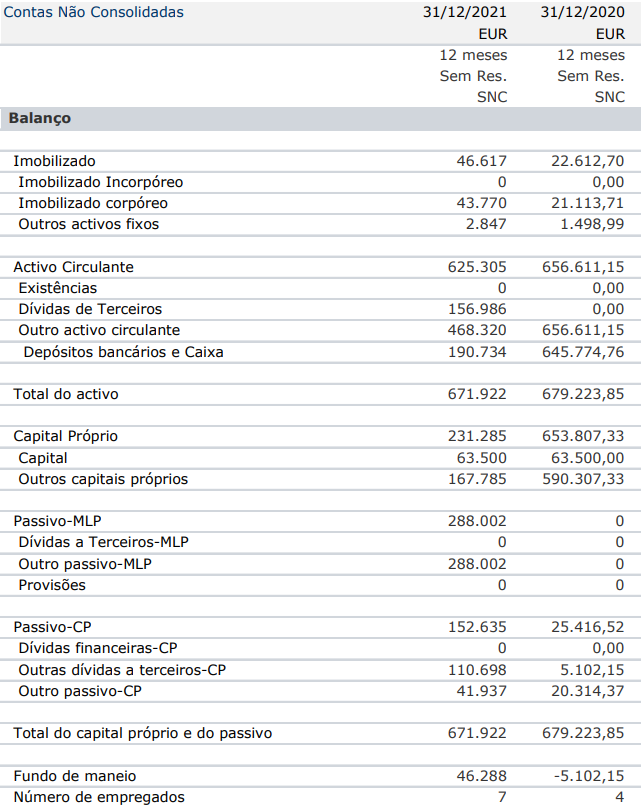
\includegraphics[width=8cm]{images/balanco_replai.png}
    \caption{Informação financeira relativa ao total do ativo, total do passivo e total do capital próprio relativo aos anos 2020 e 2021.}
    \label{fig:balanco_r}
\end{figure}

Com base nas informações apresentadas acima, é possível identificar as principais rubricas que constituem o balanço, essa demonstração é feita na figura \ref{fig:balanco_g}.\\

\begin{figure}[ht]
    \centering
    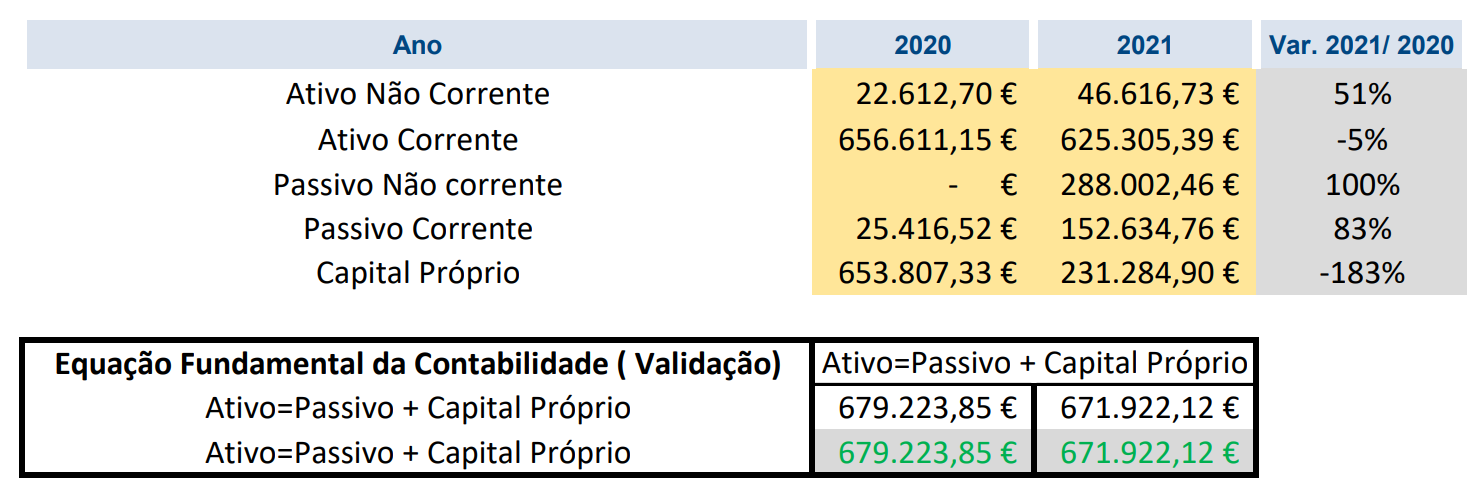
\includegraphics[width=8cm]{images/balanco_gesta.png}
    \caption{Informação financeira relativa as principais rubricas do balanço dos anos 2020 e 2021.}
    \label{fig:balanco_g}
\end{figure}

Ao examinarmos a figura \ref{fig:balanco_g} verificamos que o ativo não corrente sofreu uma variação positiva de 51\%, enquanto o ativo corrente sofreu uma variação negativa de 5\%. Já em relação ao passivo não corrente e corrente, ambos sofreram uma variação positiva, sendo essas respetivamente, de 100\% e 83\% em relação ao ano de 2020. Como os passivos corrente e não corrente sofreram uma variação considerável, e sendo essa rubrica um indicador das obrigações da empresa com terceiros, podemos concluir que houve uma variação negativa do capital próprio em 183\%, isto significa que a longo prazo se não existir uma injeção de capital na empresa a sua situação líquida poderá facilmente ser negativa.\\

Para uma avaliação mais minuciosa, iremos analisar a demonstração de resultados da empresa na figura \ref{demostracao}.
\begin{figure}[ht]
    \centering
    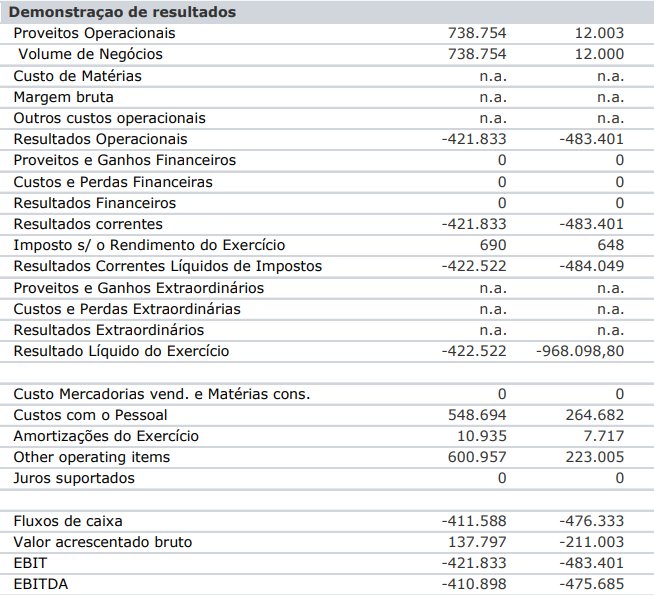
\includegraphics[width=8cm]{images/demostracao_resultados.png}
    \caption{Demonstração dos resultados relativa aos anos 2020 e 2021.}
    \label{demostracao}
\end{figure}

Ao fazer a análise da demonstração dos resultados, concluímos que o resultado líquido do período e operacional sofreram uma variação negativa de 15\% e o volume de negócio sofreu uma variação positiva de 98\%. A partir, desses valores podemos concluir que apesar do volume de venda da \textit{Replai} tem aumentado, não foi suficiente para compensar as suas dívidas que já foram referidas na análise do balanço.

\subsection{Analisar a evolução das principais rubricas do Balanço e da Demonstração dos Resultados}
É evidente que ao longo dos anos a Replai tem crescido no mercado e para o comprovar temos a análise de resultados. 


Para melhor entender esta evolução vamos então analisar o ano de 2020 e 2021.\\

Em termos de balanço, 2020 apresenta por uma margem quase nula um maior valor no Total de ativos. Neste ano a Replai também apresentou mais capital próprio comparando a 2021. 


No entanto, em 2021 a Replai demonstrou muitos melhores resultados, conseguindo acrescentar valor bruto à empresa em 137,393€ comparando aos negativos 211,003€ de 2020. 


Porém, em nenhum destes anos a Replai teve retorno, estando constantemente negativo desde 2020 em percentagem do retorno sobre o capital próprio, retorno sobre o capital investido, retorno sobre o total do ativo e margem de lucro, mesmo apesar de em 2021 quase ter atingido valores na margem de lucro e retorno sobre o total do ativo positivos. 
\newpage
\subsection{Avaliação da situação do desempenho económico-financeiro da organização usando o método dos rácios}

Esta avaliação, que é baseada no método dos rácios e consiste em calcular e comparar diferentes rácios, permite examinar o desempenho financeiro da empresa e é fundamental para tomar decisões estratégicas e garantir o sucesso da empresa no longo prazo.



\subsubsection{Situação da Tesouraria}
\textbf{Liquidez Geral}\\
\[
    \frac{\textit{Ativo Corrente}}{\textit{Passivo Corrente}} = \frac{625,305.39}{152,635.76} = 4.10
\] \\

Confirma-se que a Replai apresenta um índice de liquidez geral superior a 2, o que é considerado positivo, pois demonstra uma boa capacidade de pagamento das suas dívidas a curto prazo.

\hrulefill
\\~\\

\textbf{Liquidez Reduzida}\\
\[
    \frac{\textit{Ativo Corrente - Inventário}}{Passivo Corrente} = \frac{625,305.39 - 0}{152,635.76} = 4.10
\] \\

A Replai tem um índice de liquidez acima de 1.7, o que indica que possui uma quantidade suficiente de ativos líquidos que podem ser facilmente convertidos em caixa para satisfazer as suas obrigações financeiras a curto prazo.

A ausência de diferença entre o rácio da \textit{liquidez geral} e o rácio da \textit{liquidez reduzida} indica que a empresa não tem um elevado nível de stock, logo, não há risco associado neste fator. 


\hrulefill
\\~\\
\newpage
\subsubsection{Situação e estrutura financeira}
\textbf{Autonomia Financeira}\\

\[
    \frac{\textit{Capital Próprio}}{\textit{Ativo}} = \frac{231,284.90}{671,922.12} = 0.34
\]

Uma autonomia financeira de 0.34 significa que a Replai tem recursos suficientes para cobrir 34\% das suas despesas com os seus próprios recursos, enquanto o restante deve ser financiado por terceiros.

\hrulefill
\\~\\

\textbf{Solvabilidade}

\[
    \frac{\textit{Capital Próprio}}{\textit{Passivo}} = \frac{231,284.90}{440,638.22} = 0.52
\]

Uma solvabilidade de 0.52 significa que a empresa tem ativos suficientes para cobrir 52\% das suas dívidas, o que é considerado um nível relativamente baixo de solvabilidade. Isto representa um risco para terceiros que desejem investir na Replai, pois o capital da organização pode não ser suficiente para cobrir todo o passivo.

\hrulefill
\\~\\

\textbf{Fundo de Maneio}\\

\[
    \textit{Ativo Corrente - Passivo Corrente} = 625,305.39 - 152,635.76 = 472,669.63
\]

Podemos concluir que o facto da Replai ter 472,669.63€ no Fundo de Maneio significa que esta possui uma reserva de dinheiro suficiente para cobrir as suas despesas operacionais e outras necessidades de curto prazo. Não tendo acesso aos custos, e tendo em conta que é uma empresa pequena, também assumindo uma boa estabilidade das suas fontes de rendimento, indica que a empresa tem uma boa capacidade de gerir as suas finanças e pode estar bem preparada para lidar com pequenos imprevistos. 


\hrulefill
\\~\\
\newpage
\subsubsection{Rentabilidade}

Os seguintes rácios de rentabilidade mostram a eficiência com que a Replai gera lucro e cresce. Depois da analise destes rácios poderemos tirar a duvida anterior e verificar se as fontes de rendimento desta empresa são estáveis.\\

\textbf{Rentabilidade do Capital Próprio}\\

\[
    \frac{\textit{Resultado Liquido}}{\textit{Capital Próprio}} = \frac{-422,522.43}{231,284.90} = -1.83
\]

Tendo uma rentabilidade do capital próprio de -1.83, significa que a Replai está a perder dinheiro e que o seu património líquido está em risco.  

\hrulefill
\\~\\

\textbf{Rentabilidade do Ativo}\\

\[
    \frac{\textit{EBIT}}{\textit{Ativo Total}} = \frac{-421,832.65}{671,922.12} = -0.63
\]

O valor de -0.63 indica que a empresa está a perder dinheiro e que os seus ativos estão a perder valor. Conclui-se com isto que a Replai não está a gerar lucro e que os ativos estão em risco.

\hrulefill
\\~\\

\textbf{Rentabilidade Liquida das Vendas}\\

\[
    \frac{\textit{Resultado Liquido}}{\textit{Volume De Negócios}} = \frac{-422,522.43}{738,753.71} = -0.572
\]\\

\textbf{Rentabilidade Operacional das Vendas}\\

\[
    \frac{\textit{EBIT}}{\textit{Volume De Negócios}} = \frac{-421,832.65}{738,753.71} = -0.571
\]

Estes dois valores negativos de rentabilidade operacional e rentabilidade líquida das vendas indicam que a empresa está a perder dinheiro com as vendas, o que pode ser um sinal de problemas financeiros. Ao haver uma diferença mínima entre estes dois valores podemos concluir que a empresa tem poucos custos financeiros.


\hrulefill
\\~\\

É preciso ter em conta que estes valores podem ser resultado das condições do mercado e da estratégia de negócios da empresa. Mas tendo em conta os rácios que obtivemos podemos seguramente garantir que as fontes de rendimento da Replai não são particularmente estáveis.

\newpage
\subsection{Comentário em relação à situação económica e financeira da organização}

Estudando a informação obtida através do total ativo, passivo e do capital próprio, bem como a avaliação do desempenho económico-financeiro da organização pelos valores obtidos no método dos rácios e o balanço dos resultados obtidos, atingiu-se uma conclusão infortuna.

Comparando os valores obtidos em 2020 e 2021, o ativo corrente sofreu uma variação positiva, bem como o passivo corrente e não corrente. Porém, o ativo corrente teve uma variação negativa e, de extrema importância, o capital próprio da organização teve uma queda abrupta, rondando os -180\%.

Mesmo tendo tido taxas de rendimento drásticas no passado ano, demonstradas pelo seu crescimento no mercado, o retorno financeiro não teve dimensão suficientemente para saldar as dívidas adquiridas ao longo do período mencionado. Tal é comprovado pelo acréscimo de 137,393€ em comparação com o prejuízo de 211,003€ em 2020.\\

Tais afirmações são também comprovadas pelo método dos rácios, que demonstra uma parca autonomia financeira, baixa solvabilidade e uma rentabilidade negativa, afastando possíveis investidores. Este conjunto de fatores, torna a situação da empresa ainda mais difícil do que se encontra atualmente dado que, para tentar “reanimar” esta \textit{start-up}, seria necessária uma injeção de capital por parte de um agente externo. Porém, dado que a mesma se encontra numa árdua situação económica, os investidores são afastados desta ideia, visto que a empresa pode não conseguir sair do declínio em que se encontra desde 2020.

Esta situação frágil pode também dever-se à forma como o capital foi investido. Uma estratégia de aplicação dos fundos para o crescimento da organização com uma imagem de salvação em segundo plano possivelmente fragilizou a situação económica da Replai, permanecendo com um futuro extremamente incerto nas mãos.\\


\section{Marketing}

\subsection{Identificação da ótica adotada pela organização}

Analisando a estratégia de marketing da Replai, concluímos que a ótica utilizada é a de Marketing.

Atualmente, sendo a publicidade uma componente do Marketing, é importante poder maximizar o seu potencial e efetividade. Ironicamente, todo o propósito da Replai é também permitir às empresas atingir esse objetivo.
  
De forma a poderem chegar aos seus clientes, estes anunciam que o seu produto, para além de fornecer estatísticas consoante as submissões de conteúdo efetuadas, permite também obter recomendações personalizadas de forma a incrementar a taxa de visibilidade dos conteúdos.
  
Ao oferecer este grau de adaptabilidade e personalização, acrescentam imenso valor ao seu produto, pois vai de encontro às necessidades de quem o subscreve. Assim, conseguem manter-se competitivos e inovadores num mercado em constante evolução.\\

\newpage
\subsection{Identificação do(s) segmento(s) de mercado e das suas características}

A \textit{Replai} opera no mercado de desenvolvimento tecnológico, o seu nicho de mercado mais específico é a utilização de inteligência artificial para otimização do trabalho que anteriormente era feito de forma manual.\\

Sendo a empresa uma \textit{StartUp}, optou por um público-alvo empresarial, segmentando o seu nicho de mercado para relações apenas com pessoas jurídicas, para além dessa característica, procura clientes internacionais, e para uma melhor integração contrata colaboradores que falem a língua nativa do país ao qual estão tentando adquirir como parceiro.\\

\subsection{Identificar o posicionamento da marca e/ou dos produtos}
O posicionamento do produto/marca consiste na forma como um produto/marca é visto pelos consumidores, isto é, o lugar que o produto/marca ocupa na mente dos consumidores em relação aos produtos concorrentes.\\

O produto da Replai é visto para o consumidor como um produto exclusivo, evolucionista e criativo: "We are replai, Revolutionizing the way we leverage creative data". Desta forma, apesar de serem uma marca relativamente recente no mercado, o seu posicionamento já permite que sejam uma marca respeitada, forte e única. 

\subsection{Marketing-mix}

\subsubsection{Produto}

A Replai tem um único produto, é uma inteligência artificial que analisa vídeos e devolve feedback sobre os mesmos, ao contrário de outros produtos neste mercado, o produto da Replai também diz ao cliente como melhorar o vídeo. Este produto é único e oferece uma vantagem competitiva para a empresa em relação aos seus concorrentes.


\subsubsection{Preço}

 É verdade que a Replai tem um dos produtos mais caros no mercado, se não o mais caro, mas este preço é justificado pelo que o produto oferece em comparação com outras opções no mercado. Se o cliente deseja a melhor qualidade de resultados, não tem muitas outras opções a não ser a Replai.

No entanto, é importante notar que a Replai não tem lucro nas suas vendas. Isso pode ser um desafio para a empresa, pois a sustentabilidade financeira é crucial para o sucesso a longo prazo. A Replai pode precisar encontrar maneiras de aumentar o preço do produto ou reduzir seus custos para garantir que continue a operar de forma eficiente e rentável.

\subsubsection{Distribuição}

No caso da Replai, os clientes fazem subscrição anual e recebem os resultados em forma digital, ou seja, a distribuição do produto é principalmente online (e-commerce). É importante que a Replai ofereça uma boa experiência de compra e entrega para garantir a satisfação dos clientes e promover a fidelidade à marca, e esta forma de entrega de resultados é a melhor para este mercado.


\subsubsection{Comunicação}

A Replai depende muito das relações públicas para se expor ao seu público-alvo, mas devido à dimensão do mercado, qualquer empresa interessada neste tipo de produtos pode facilmente encontrá-la.

\section{Gestão das Operações e Indústria 4.0}

\subsection{Operações de produção que a Replai desenvolve}

A Replai produz um serviço de inteligência artificial que analisa vídeos e devolve estatísticas utilizando tecnologias avançadas de \textit{machine learning} e análise de dados. 

Para desenvolver este serviço, a organização conta com uma equipa de programadores e especialistas destas tecnologias que trabalham em sintonia usando metodologias ágeis, como \textit{sprints} e \textit{scrum}, para garantir o sucesso do projeto. Além disso, a Replai possui um departamento de pesquisa cujo objetivo é trazer informações que sejam centradas no cliente, ou seja, descobrir o que o cliente realmente quer e como o serviço pode ser aperfeiçoado para atender às suas necessidades. Esta é a única operação de produção da Replai, que se foca em fornecer este serviço aos seus clientes.\\

\subsection{Identificação dos principais elementos da cadeia de abastecimento da organização}
  
Desconstruindo o conjunto de processos da cadeia de abastecimento da Replai, foi-nos possível concluir que esta é extremamente curta, porém, com a capacidade de acrescentar imenso valor e deveras eficiente.

Vendo a sequência desde a primeira interação até ao produto final, na sua gestão de operações de produção, podemos considerar como fornecedores os seus clientes, como organizações privadas (Zynga ou TapNation, por exemplo), através das subscrições.
  
No seu ambiente, ocorre uma análise por parte do algoritmo, bem como a criação de recomendações personalizadas, surgindo aqui o valor do serviço que fornecem, que mais tarde será output em forma de informação e \textit{know-how}. 

Contudo, como se trata de um processo inteiramente digital, excetuando componentes de interação com o cliente, também digitais, não existe qualquer processo logístico associado.

Assim, baseia-se na subscrição do serviço e na entrega dos dados gerados, originando uma cadeira inversamente proporcional às cadeias de indústrias habituais.

\subsection{Identificar o tipo de sistema produtivo adotado na organização.}

Depois de uma análise e reflexão sobre os cinco tipos de processos produtivos quanto ao mercado, sendo eles, produção por projeto, unitária ou \textit{Job Shop}, por lotes, em série ou massa, e em contínuo. \\

Consideramos que a que melhor se enquadra no perfil da \textit{Replai} é a produção por encomenda. Visto que, a empresa apesar de usar a mesma ferramenta para todos os projetos desenvolvidos, sendo essa, o algoritmo desenvolvido pelos seus colaboradores, cada projeto contém as suas especificidades e gera um resultado único para cada cliente. \\

Já do ponto de vista da relação da produção com o cliente, consideramos que o tipo de produção que melhor enquadra-se com a empresa é a produção por encomenda, visto que, um projeto inicia-se apenas quando existe um acordo já predefinido entre a empresa e o seu cliente alvo. \\

\subsection{Relacionar a organização da produção com as opções de marketing }
No caso da Replai, que opera a produção por projeto, é essencial para o seu sucesso adotarem uma ótica de marketing, pois o mercado onde estes estão inseridos é bastante competitivo e suscetível a tendências. \\

Assim, torna-se essencial identificar e recolher os requisitos que os clientes mais procuram e/ou sentem falta no produto, para que o valor associado à marca da Replai se mantenha ou até melhore. Esta fase de recolha de requisitos é das fases mais cruciais quando se trata de produção por projeto, pois o planeamento do projeto precisa ser extenso e detalhado para que o resultado encontre as necessidades do mercado. 

\subsection{KPI’s de gestão de operações de produção na organização.}
Para analisar e gerir as operações de produção no produto da Replai, utilizam-se alguns dos KPI’s mencionados no ponto 2.4.3., principalmente as ferramentas de aquisição, de compromisso e retenção. Estes KPI’s visam perceber a percentagem de novos utilizadores sobre a percentagem de pessoas que procura o produto, o número de utilizadores ativos sobre o número de utilizadores totais e o tempo de subscrição média na plataforma por cliente, respetivamente. 

\subsection{Tecnologias utilizadas pela Replai para a recolha e tratamento de dados das operações de produção.}

A Replai produz um único serviço que consiste na recolha e tratamento de dados. Este serviço consiste em analisar vídeos e retornar estatísticas aos seus clientes. Para tratar os dados dos vídeos, a Replai utiliza \textit{Machine Learning}, que consiste em desenvolver algoritmos e modelos que podem aprender com os dados e melhorar a precisão das suas previsões e decisões. Ao utilizar esta tecnologia, a Replai extrai informações valiosas dos vídeos e fornece estatísticas mais precisas e relevantes aos seus clientes. A Replai pode usar esta tecnologia para aperfeiçoar continuamente o seu serviço, treinando os seus modelos com novos dados dos vídeos para aumentar a sua precisão e desempenho. Isso permite que a Replai ofereça um serviço cada vez mais eficiente e adaptado às necessidades dos seus clientes.

\subsection{Utilização de tecnologias da indústria 4.0}

De forma a poder manter-se a par dos mais recentes breakthroughs que a revolução da Indústria 4.0 trouxe, a Replai adota inovações que são chave para o funcionamento do produto que a empresa fornece aos seus subscritores. Vamos ver:\\

•	Big Data: O algoritmo usado para realizar a análise e gerar as estatísticas dos vídeos submetidos é, como mencionado previamente, baseado em Machine Learning, que necessita de uma grande quantidade de dados de forma a poder dar respostas precisas e adequadas ao contexto de negócio em que se insere.\\

•	Advanced Analytics: Para tomar alguma forma de decisão, é importante basear as escolhas efetuadas num portefólio de informação previamente registada. Para tal, alia-se a funcionalidade de Big Data com esta, originando uma poderosa ferramenta de poder decisão, implicando positivamente a forma como o algoritmo da Replai retornará o feedback ao subscritor do serviço. Assim, aumento a taxa de fidedignidade do seu produto e, para além disso, permite tornar mais robusto o alicerce de funcionamento.\\

•	Cloud Computing: Para uma empresa de dimensão tão reduzida e com clientes de dimensões inversamente proporcionais, é deveras importante existir uma elevada capacidade de computação para conseguir servir todos de forma eficaz e eficiente. Contudo, hardware próprio, como servidores, é extremamente caro de manter, requer um forte investimento inicial e uma constante necessidade de aumentar a capacidade do mesmo. Num contexto económico frágil, serviços de computação na cloud, como os que são fornecidos pela AWS (Amazon Web Services, usados pela empresa)  permitem a pequenas organizações ter as suas demandas de processamento satisfeitas através de uma subscrição, tornando esta solução ideal.